\chapter{Background}
\label{chapter:background}

This chapter introduces key concepts related to \glsxtrfull{vqa}. Given the multimodal nature of this task, we present concepts from \gls{nlp} and computer vision separately, followed by a detailed exploration of their integration in \glspl{vlm}. In the natural language section, we focus on \glspl{rnn} and the transformer architecture, while for the computer vision section, we focus on \glspl{cnn} and \glspl{vit}. Then, a historical approach is adopted to delve into \gls{vqa} architectures and datasets.

\newpage


\section{Natural Language Processing, Understanding and Generation}

This section delves into key concepts of \gls{ai} applied to written language. It begins by clarifying the distinctions between \gls{nlp}, \gls{nlu}, and \gls{nlg}. Next, it examines essential processing steps like tokenization and word embeddings. Finally, the section explores crucial architectural developments like \glspl{rnn}, \gls{lstm} networks, and transformers, concluding with a brief introduction to \glspl{llm}.

\subsection{NLP vs. NLU vs. NLG}

The topics of \gls{nlp}, \gls{nlu} and \gls{nlg}, though related, are understood to mean different things. Broadly speaking, \gls{nlu} and \gls{nlg} are sub-topics of \gls{nlp} (See Fig.~\ref{fig:nlp_nlu_nlg}), as described in the following definitions~\cite{ibmNLGDifferences,datasolutNLGUnterschiede}:

\begin{figure}[!ht]
\begin{center}
\includegraphics[width=0.70\textwidth]{Figures/Background/nlp_nlu_nlg.pdf}
\caption{Relationship between NLP, NLU and NLG.}
\label{fig:nlp_nlu_nlg}
\end{center}
\end{figure}

\begin{itemize}
    \item \textbf{\glsxtrfull{nlp}: } Rooted in computational linguistics, \gls{nlp} comprises a wide range of operations applied to text. Its central aim is to add structure to text to endow computers with the ability to process it and generate responses.
    \item \textbf{\glsxtrfull{nlu}: } Delving deeper into textual meaning, \gls{nlu} is concerned with the meaning of the text in terms of comprehension of grammar and context. Key features include part-of-speech tagging (adjectives, verbs, \etc), grammatical case recognition, and keyword identification.    
    \item \textbf{\glsxtrfull{nlg}: } Shifting the focus to generating text, \gls{nlg} focuses on the generation of text in English or other languages. It encompasses tasks such as natural language generation, summarization, and translation.
\end{itemize}

\subsection{Tokenization}

Humans primarily use variable-length words arranged in sequences for language representation. Each word, encoded using standards like ASCII or UTF-8~\cite{rao2019natural}, comprises a sequence of alphanumeric characters. Sentences and paragraphs remain unstructured data. To obtain structured data that is manipulable by computers, a process called tokenization breaks the text into discrete pieces. These pieces, known as tokens, can be words, subwords, or characters, depending on the desired granularity.



\subsection{Word Embeddings}

Word embeddings represent tokens as numerical vectors in a high-dimensional space. Given a sequence $\T = [w_1,w_2, ..., w_n]$ of $n$ tokens, the embedding of the i-th word or token is denoted $E(w_i)$. The function $E$ transforms the token $w_i$ into a fixed-size, real-valued vector representation, allowing syntactically or semantically similar tokens to have comparable representations. Thus, the word embeddings can be represented as

\begin{equation}
    \mathbf{WE} = [E(w_1), E(w_2), ..., E(w_n)] \in \real ^ {n \times J},
\end{equation}

where $J$ is the dimension of each word embedding vector. 

Some popular techniques to obtain word embeddings include \gls{bow}~\cite{sivic2008efficient}, Word2Vec~\cite{mikolov2013efficient}, GloVe~\cite{pennington2014glove} and BERT~\cite{devlin2018bert}.

\subsection{Recurrent Neural Networks}

\glspl{rnn}~\cite{rumelhart1986learning} are networks that process sequential data. To understand the concept better, it is useful to start from the formulation of a dynamical system, as presented in~\cite{goodfellow2016deep}, where a function $f$ parameterized by $\bm{\theta}$ is applied to the previous state,

\begin{equation}
    \mathbf{h}^{(t)} = f(\mathbf{h}^{(t-1)}; \bm{\theta}),
    \label{eq:dynamical_system}
\end{equation}

where $\mathbf{h}$ is the state of the system. This equation is said to be recurrent because the value of the state $\mathbf{h}$ at time $t$ depends on its value at time $t-1$. For a given finite value of $t$, unfolding the graph that Eq.~\eqref{eq:dynamical_system} represents is possible. This is, the equation is applied multiple times in a recurrent way to obtain a non-recurrent expression. For example, for $t=3$,

\begin{equation}
    \mathbf{h}^{(3)} = f(f(\bm{h}^{(1)}; \bm{\theta}); \bm{\theta}),
\end{equation}

which reveals the function being applied multiple times in a sequential manner. This can be represented with a graph, as shown in Fig.~\ref{fig:unfolded_graph}, where each node represents a hidden state, and the edges represent the function. 

\begin{figure}[!ht]
\begin{center}
\includegraphics[width=0.60\textwidth]{Figures/Background/unfolded_graph.pdf}
\caption{Unfolded graph for Eq.~\eqref{eq:dynamical_system}. Based on~\cite{goodfellow2016deep}.}
\label{fig:unfolded_graph}
\end{center}
\end{figure}

Including an external signal or input $\s$ results in a recurrent network, which can be represented by
\begin{equation}
    \h^{(t)} = f(\h^{(t-1)}, \, \s^{(t)}; \bm{\theta}),
    \label{eq:rnn}
\end{equation}
 whose unfolded version is depicted in \fig~\ref{fig:unfolded_rnn} with the outputs $\mathbf{o}$ for each state.
 
\begin{figure}[!ht]
\begin{center}
\includegraphics[width=0.80\textwidth]{Figures/Background/unfolded_rnn_full.pdf}
\caption{Unfolded RNN for Eq.~\eqref{eq:rnn}. Based on~\cite{goodfellow2016deep}.}
\label{fig:unfolded_rnn}
\end{center}
\end{figure}

One limitation of \glspl{rnn} is the challenge in considering long-term dependencies in the input data. This issue arises from the exponentially smaller weights assigned to these long-term interactions (\ie, vanishing gradient). For instance, consider the case in which the network is tasked with predicting the subsequent words in the sentence, "John is allergic to nuts. He refused to try the..." In this scenario, the context provided by the first sentence (nut allergy) aids in predicting more accurate words. However, if this context is situated at a greater distance from the word to be predicted, the network might struggle to utilize it effectively. A second issue is the occurrence of exploding gradients, leading to model instability and affecting the training process. Another constraint of the presented \gls{rnn} is its unidirectional nature, limiting its capacity to incorporate future events for predicting more meaningful states~\cite{ibmWhatRecurrent}. We now present some variations that attempt to tackle these limitations.


\subsubsection{RNN Variations}
% https://www.ibm.com/topics/recurrent-neural-networks
We examine the most common variations of \glspl{rnn}

\begin{itemize}
    \item \textbf{\glsxtrfull{brnn}\cite{schuster1997bidirectional}:} In certain applications, like speech and handwriting recognition, generating an output that depends on all the input sequence elements can be beneficial. \glspl{brnn} tackle this by merging two \glspl{rnn}: one that begins at the initial sequence element and progresses forward, and another that commences at the final sequence element and progresses backward (refer to \fig~\ref{fig:brnn}). This network configuration allows for outputs that take into account both past and future elements but are particularly sensitive to inputs near time step $t$.

    \begin{figure}[!ht]
    \begin{center}
    \includegraphics[width=0.40\textwidth]{Figures/Background/brnn.pdf}
    \caption{Unfolded BRNN. Based on~\cite{goodfellow2016deep}.}
    \label{fig:brnn}
    \end{center}
    \end{figure}

    
    \item \textbf{\glsxtrfull{lstm}~\cite{hochreiter1997long}:} Arguably the most popular \gls{rnn} architecture, it was introduced as a solution to the vanishing gradient issues of vanilla \glspl{rnn}. Consequently, this architecture handles long-term dependencies more effectively. As illustrated in \fig~\ref{fig:lstm}, the \gls{lstm} mitigates the long-term dependency problem by using a cell state and incorporating three types of gates: input, output, and forget. These gates facilitate control over the flow of information within the network. The cell, depicted in \fig~\ref{fig:lstm}, comprises a cell state and a hidden state. The forget gate filters out irrelevant information from the previous cell state $\mathbf{C}^{(t-1)}$, such as a gender mentioned multiple times in the preceding sentences. Subsequently, the input gate determines which new information should be added to the current cell state $\mathbf{C}^{(t)}$. Finally, the output gate determines which information from the current cell state should be incorporated into the current hidden state $\mathbf{h}^{(t)}$.
    \begin{figure}[!ht]
    \begin{center}
    \includegraphics[width=0.60\textwidth]{Figures/Background/lstm.pdf}
    \caption{LSTM cell diagram.}
    \label{fig:lstm}
    \end{center}
    \end{figure}

    Equations~\eqref{eq:lstm_first}-\eqref{eq:lstm_last} define the behaviour of each \gls{lstm} cell. Here, $\bm{U}_f$, $\bm{U}_i$, $\bm{U}_o$, $\bm{U}_g$, $\bm{W}_f$, $\bm{W}_i$, $\bm{W}_o$ and $\bm{W}_f$ correspond to learnable parameters of linear mappings, and $\odot$ is the element-wise product.

    \begin{equation}
        \bm{f}^{(t)} = \sigma \left( \s^{(t)}\bm{U}_f + \bm{h}^{(t-1)}\bm{W}_f \right)
        \label{eq:lstm_first}
    \end{equation}
    \begin{equation}
        \bm{i}^{(t)} = \sigma \left( \s^{(t)}\bm{U}_i + \bm{h}^{(t-1)}\bm{W}_i\right)
    \end{equation}
    \begin{equation}
        \bm{o}^{(t)} = \sigma \left( \s^{(t)}\bm{U}_o + \bm{h}^{(t-1)}\bm{W}_o\right)
    \end{equation}
    \begin{equation}
        \tilde{\bm{C}}^{(t)} = tanh \left( \s^{(t)}\bm{U}_g + \bm{h}^{(t-1)}\bm{W}_g\right)
    \end{equation}
    \begin{equation}
        \bm{C}^{(t)} = \sigma \left( \bm{f}^{(t)} \odot \bm{C}^{(t-1)} + \bm{i}^{(t)} \odot \tilde{\bm{C}}^{(t)}\right)
    \end{equation}
    \begin{equation}
        \bm{h}^{(t)} = tanh \left( \bm{C}^{(t)}\right) \odot \bm{o}^{(t)}
        \label{eq:lstm_last}
    \end{equation}

    
    \item \textbf{\glsxtrfull{gru}~\cite{cho2014learning}:} This architecture also focuses on mitigating the long-term dependency issues of \glspl{rnn}. Unlike the \gls{lstm}, \glspl{gru} do not make use of a cell state to control the information flow. It uses hidden states and has two gates (reset and update). 


\end{itemize}



\subsection{The Transformer Architecture}
\label{sec:transformer}
% describe

The transformer architecture~\cite{vaswani2017attention} was introduced in 2017. Since its inception, this architecture has been applied in various domains, including language processing and computer vision. The utilization of transformers in image processing is further discussed in Sec.~\ref{subsec:vit}. As previously mentioned, recurrent neural networks have limitations, including the absence of parallelization, which hinders efficiency, and issues related to long-term dependencies due to vanishing and exploding gradients. The transformer addresses these limitations through its attention mechanism and architectural design.

The transformer, as depicted in Fig.~\ref{fig:transformer_architecture}, follows an encoder-decoder structure. In this setup, the input text undergoes mapping to a representation space by the encoder. Subsequently, the decoder utilizes this representation to sequentially generate an output sequence. This process is termed \textit{auto-regressive} behavior because, at each time step, the previously generated elements serve as input for producing a new one.

\begin{figure}[!ht]
\begin{center}
\includegraphics[width=0.55\textwidth]{Figures/Background/transformer_architecture.png}
\caption{Transformer architecture. From~\cite{vaswani2017attention}.}
\label{fig:transformer_architecture}
\end{center}
\end{figure}

\subsubsection{Encoder}

The encoder block, illustrated in Fig.~\ref{fig:transformer_architecture}, is responsible for generating a continuous representation from the embedded and positionally encoded inputs. The encoder consists of two sub-layers: a multi-head self-attention mechanism and a feed-forward network. Following~\cite{he2016deep}, residual connections are incorporated into each sub-layer, along with layer normalization~\cite{ba2016layer}. Instead of having one single encoder layer, the encoder is structured as a stack of six identical layers.

\subsubsection{Decoder}

The decoder block shares certain similarities with the encoder: It is constructed as a stack of six layers, employs residual connections and layer normalization, and incorporates both multi-head attention and a fully connected network. Nevertheless, it diverges by featuring two multi-head attention sub-layers instead of one. The second sub-layer serves the specific function of processing the output of the encoder. As depicted in Fig.~\ref{fig:transformer_architecture}, the sub-layer responsible for receiving the previously generated outputs incorporates a masking mechanism, preventing the model from attending to future positions.

\subsubsection{Attention}

The key part of the transformer architecture is its self-attention mechanism. The concept of \textit{attention} was initially introduced in~\cite{bahdanau2014neural} for machine translation. The basic idea was to enable the model to determine which parts of the source sentence were relevant to predict the next word of the translation. In the transformer, the attention function is expressed in terms of three elements: queries, keys, and values, all represented as vectors. The output is computed by taking the weighted sum of the values, with each value assigned a weight determined by a compatibility function between the query and its corresponding key. Put differently, the transformer uses the self-attention mechanism to consider other words relevant to the word currently being processed. For instance, in translating the sentence "The cat climbed the bed because it was tired," self-attention allows the model to recognize that the word "it" is more closely associated with the word "cat" than with any other word in the sentence~\cite{jalammarIllustratedTransformer}.

The transformer's implementation of the self-attention mechanism is called scaled dot-product attention and is illustrated in Fig.~\ref{fig:attention_transformer} (A). In this process, the dot products are computed between the query and all keys, then scaled by the dimension of the keys, $d_k$, and finally, a softmax function assigns weights of the values. This operation can be performed for a set of queries efficiently using matrices. Denoting the matrices $\bm{Q}$, $\bm{K}$, and $\bm{V}$ for queries, keys, and values, respectively, the attention operation is defined by Eq.\eqref{eq:attention}.
 
\begin{equation}
    \text{Attention}(\bm{Q}, \bm{K}, \bm{V})  = softmax \left( \frac{\bm{Q}\bm{K}^T}{\sqrt{d_k}} \right) \bm{V}
    \label{eq:attention}
\end{equation}

\begin{figure}[t]
\centering
\begin{subfigure}{.42\textwidth}
  \centering
  \includegraphics[width=.4\linewidth]{Figures/Background/scaled_dot_product_att.png}
  \caption{Scaled dot-product attention block.}
  \label{fig:sub1}
\end{subfigure}%
\begin{subfigure}{.5\textwidth}
  \centering
  \includegraphics[width=.6\linewidth]{Figures/Background/multi_head_att.png}
  \caption{Multi-head attention.}
  \label{fig:sub2}
\end{subfigure}
\caption{Self-attention modules of the transformer architecture. From~\cite{vaswani2017attention}.}
\label{fig:attention_transformer}
\end{figure}

As shown in Fig.~\ref{fig:attention_transformer} (B), self-attention is performed for $h$ ``heads" $\{\bm{z_1}$, $\bm{z_2}$, ..., $\bm{z_h}\}$, projecting the queries, keys, and values with learned linear functions. This enables the simultaneous application of scaled dot-product attention on each head, producing output values with dimension $d_v$. Subsequently, these output values are concatenated and projected once again,

\begin{equation}
    \text{MultiHead}(\bm{Q},\bm{K},\bm{V}) = Concat(\bm{z_1}, ..., \bm{z_h}) \bm{W}^O
\end{equation}

where 

\begin{equation}
\bm{z_i} = \text{Attention}(\bm{Q}\bm{W_i^Q},\bm{K}\bm{W_i^K},\bm{V}\bm{W_i^V})
 \end{equation}

with $\bm{W}$ representing the learnable parameters of the projection layers.

\subsubsection{Positional Encoding}

Positional encodings are necessary due to the lack of recurrence and convolutions so the model can consider the order of the input sequence. In the transformer architecture, positional encodings are added to the input embeddings for both the encoder and decoder blocks. Sine and cosine functions are used to this end, as follows

\begin{equation}
    \bm{PE}_{(pos, \, 2i)} = sin \left( \frac{\bm{pos}}{10000^{\frac{2i}{d_{\text{model}}}}} \right)
\end{equation}
\begin{equation}
    \bm{PE}_{(pos, \, 2i+1)} = cos \left( \frac{\bm{pos}}{10000^{\frac{2i}{d_{\text{model}}}}} \right)
\end{equation}

where $\bm{pos}$ represents the position and $i$ the dimension. In other words, each dimension of the positional encoding represents a sinusoidal function, and the wavelengths exhibit a geometric progression ranging from $2\pi$ to $10000 \cdot 2\pi$.

\subsection{Large Language Models}

% show plot from I don't know where to show evolution of huge models, i.e., time vs. number of parameters

\glspl{llm} can be defined as very deep transformer-based models optimized for one or multiple language tasks using internet-scale datasets. These models can easily reach hundreds of billions of parameters. In fact, as illustrated in \fig~\ref{fig:llm_size_trend}, there is a noticeable upward trend in model size. For instance, in June 2020, OpenAI unveiled GPT-3, which featured 175B parameters and was able to generate text and code with short prompts written by the user~\cite{brown2020language,nvidiaWhatLarge}. One year later, Megatron-Turing NLG, with 530B parameters, was introduced~\cite{smith2022using}. The number of parameters for more recent models such as GPT-4~\cite{achiam2023gpt} has not been disclosed, but it is believed to exceed one trillion parameters.


\begin{figure}[!ht]
\begin{center}
\includegraphics[width=0.6\textwidth]{Figures/Background/llm_size_trend.pdf}
\caption{LLM size versus time. Adapted from~\cite{nvidiaUsingDeepSpeed}.}
\label{fig:llm_size_trend}
\end{center}
\end{figure}


\subsubsection{Types}
% encoder only, decoder only, encoder-decoder
As mentioned in Sec.~\ref{sec:transformer}, the transformer architecture comprises an encoder and a decoder. Nevertheless, not all implementations based on this architecture adhere strictly to this design. In general, depending on the task at hand, \gls{llm} can be categorized into the following groups~\cite{nvidiaWhatLarge}:

\begin{itemize}
    \item \textbf{Encoder only:} Models typically employed for tasks involving language understanding but without text generation as output. In such instances, the encoder is responsible for producing meaningful representations of the input, utilized by another network block, such as a classification head. Tasks like classification and sentiment analysis fall within this category. An example of this model type is \glsxtrshort{bert}~\cite{devlin2018bert}.

    \item \textbf{Decoder only:} These models are designed to generate high-quality language and content suitable for tasks such as blog generation and storytelling. GPT-3~\cite{brown2020language} is an exemplar of this model type. 

    \item \textbf{Encoder-decoder:} This model can both understand and generate text. Use cases include tasks like text translation and summarization. T5~\cite{raffel2020exploring} is an example of an architecture that utilizes an encoder-decoder structure.
\end{itemize}

\subsubsection{Applications}

\glspl{llm} can be used for diverse tasks. \fig~\ref{fig:llm_applications} shows the five main use case categories. For each category, some specific examples are provided. 

\begin{figure}[!ht]
\begin{center}
\includegraphics[width=0.6\textwidth]{Figures/Background/llm_applications.pdf}
\caption{Applications of LLMs. Based on~\cite{nvidiaWhatLarge}.}
\label{fig:llm_applications}
\end{center}
\end{figure}

In the medical domain, \glspl{llm} have demonstrated diverse applications, including radiology report summarization~\cite{van2023clinical}, medical record evaluation~\cite{schubert2023large}, drug discovery~\cite{pal2023chatgpt}, and others. Noteworthy breakthroughs have also been made in the field of robotics~\cite{ma2023eureka}. When equipped with vision capabilities (see Sec.~\ref{subsec:mllms}), \glspl{llm} extend their applications to include radiology report generation~\cite{wang2023r2gengpt}, surgical training~\cite{varas2023innovations,mohapatra2023leveraging}, patient education~\cite{mesko2023impact}, assistive technologies for visually impaired people~\cite{wu2023multimodal}, and autonomous driving~\cite{cui2024survey}, among others. 

\subsubsection{Challenges}

Due to the large scale of both models and datasets, \glspl{llm} brings about special challenges that require consideration~\cite{nvidiaWhatLarge}:

\begin{itemize}
    \item \textbf{Training cost:} The large scale of \glspl{llm} entails higher training requirements in terms of computing, capital and time, not only during development but also for deployment and maintenance. For example, the training of BLOOM, an open-source \gls{llm} with 176B parameter, took about 2.5 months, consumed 1,082,990 compute hours, and utilized 48 nodes with 8 Nvidia A100 80GB GPUs~\cite{workshop2022bloom}. For GPT-3, it is estimated that the cost of training was over USD 12 million~\cite{forbesCouncilPost}.

    \item \textbf{Scale of data:} \glspl{llm} require a substantial volume of data for training. In some cases, obtaining the data can be difficult due to privacy concerns (\eg, medical data). In general, the curation of such extensive datasets poses a challenge in itself.

    \item \textbf{Technical expertise:} Given the large scale of the models, both training and deployment demand a certain level of expertise in areas such as deep learning pipelines, architectures, distributed computing, \etc
    
\end{itemize}

Due to these challenges, a set of methods has been proposed for fine-tuning \glspl{llm}, by minimizing the number of parameters that are modified. This provides advantages for researchers, institutions, and companies lacking the necessary infrastructure to properly fine-tune the model for a downstream task or a specific dataset. This set of methods is referred to as \gls{peft}. Some of the most popular techniques include Adapters~\cite{houlsby2019parameterefficient}, LoRA~\cite{hu2021lora}, and prefix tuning~\cite{li2021prefixtuning}. %, but the amount of methods has been increasing in recent years, as shown in \fig~\ref{fig:peft}. 


%\begin{figure}[!h]
%\begin{center}
%\includegraphics[width=\textwidth]{Figures/Background/peft.png}
%\caption{Evolution of PEFT in recent years. From~\cite{xu2023parameterefficient}.}
%\label{fig:peft}
%\end{center}
%\end{figure}


\section{Computer Vision}

This section briefly presents some essential computer vision concepts, with a focus on \glspl{cnn} and \glspl{vit}, as they are the most relevant architectural types for this work.

\subsection{Convolutional Neural Networks}

\glspl{cnn} are networks designed to process data represented in a 2D structure, such as images and time series. As its name indicates, \glspl{cnn} employ a mathematical operation known as convolution, which is a specialized type of linear operation. Thus, \glspl{cnn} can be characterized as neural networks that apply convolution in certain layers~\cite{goodfellow2016deep}. This operation takes place between the input and a convolution kernel. Rather than providing the continuous and 1D discrete definitions, we present the 2D convolution definition between an image $\x$ and a kernel $\mathbf{k}$:

\begin{equation}
    \bm{S}(i,j) = (\x*\bm{k})(i,j) = \sum_m \sum_n \x(m,n)\bm{k}(i-m, j-n)
    \label{eq:convolution}
\end{equation}

where the indices $m$ and $n$ represent the valid positions for the operation. Eq.~\eqref{eq:convolution} indicates that the convolution operation is performed at every pixel location $i,j$ of the image. With a kernel smaller than the input image, \glspl{cnn} implement sparse interactions, implying that not every element of the output needs to be determined by every element of the input. This approach offers advantages in terms of efficiency and memory requirements.

\glspl{cnn} are typically arranged in sequential convolutional layers, where the output of each layer undergoes processing by a subsequent layer. The output of each layer is commonly referred to as a feature map, as different layers extract image features at various levels of abstraction (such as edges, objects, etc.). Convolutional layers usually consist of three components: 

\begin{itemize}
    \item \textbf{Convolution block:} The input is convolved with $h$ kernels to produce $h$ feature maps.

    \item \textbf{Non-linearity block:} Applying a non-linearity or activation function enables the model to learn more complex functions. Some common non-linearities used in \glspl{cnn} include \gls{relu}, leaky ReLU, and \gls{gelu}~\cite{dubey2022activation}.

    \item \textbf{Pooling block:} Enables the reduction of the output size by summarizing each location through a statistic involving several neighboring values. For instance, the max pooling operation~\cite{gholamalinezhad2020pooling} defines each value as the maximum value in a rectangular sub-region.
    
\end{itemize}


%\subsubsection{ResNet}?



\subsection{Vision Transformers}
\label{subsec:vit}
The Vision Transformer (\gls{vit}) extends the transformer architecture to handle images. As discussed in Sec.~\ref{sec:transformer}, the transformer operates on token vectorial representations, which are readily obtained for text through tokenization and token embeddings. The most effective equivalent of tokens for images and processing pipeline remained unclear until 2020 when the \gls{vit} was introduced~\cite{dosovitskiy2020image}. 

The core idea of the \gls{vit} involves dividing the image into fixed-size tiles or patches, treating these as tokens, as depicted in~\fig~\ref{fig:vit}. The patches need to be flattened first and then linearly projected to a constant latent vector dimension $D$. Then, positional embeddings are added to retain the information about the relative position of each patch. The result of this is processed by a transformer encoder block, which differs from the original transformer block in that the layer normalization is applied before every block instead of after (refer to~\fig~\ref{fig:transformer_architecture}). Since the \gls{vit} was introduced for image classification, the authors use a classification head at the model's output and leverage a learnable embedding prepended to the sequence of projected patches. This learnable embedding acts as image representation, following ideas proposed previously for \glsxtrshort{bert}. Two popular versions of \glspl{vit} are Swin Transformers~\cite{liu2021swin} and DeiT~\cite{touvron2021training}, which focus on scalability and data efficiency, respectively.

\begin{figure}[ht]
\begin{center}
\includegraphics[width=\textwidth]{Figures/Background/vit.png}
\caption{Vision Transformer (ViT) architecture overview. \textbf{Left:} General ViT pipeline. \textbf{Right:} Transformer encoder design. From~\cite{dosovitskiy2020image}.}
\label{fig:vit}
\end{center}
\end{figure}

\section{Vision-Language Models}

Models that integrate both vision and language capabilities are referred to as \glspl{vlm}. The typical \gls{vlm} structure consists of a vision encoder, a text encoder, and a strategy or mechanism to combine the two. During the training process using text and image data, the features of both modalities are expected to ``align," signifying that the model learns representations that reveal the correspondence between text and vision, contributing to improved outputs. Tasks addressed by \glspl{vlm} encompass:

\begin{itemize}
    \item \textbf{Image retrieval:} Determining the most suitable image in a dataset that best corresponds to an input sentence~\cite{lee2018stacked}.

    \item \textbf{Visual grounding:} Matching the words in an input sentence to the corresponding objects in an image~\cite{kazemzadeh2014referitgame}.

    \item \textbf{Visual Question Answering:} Generating an appropriate answer to a question about an image~\cite{antol2015vqa}. Due to its significance in this work, a more detailed overview of this task is provided in Sec.~\ref{sec:vqa_background}.

    \item \textbf{Image captioning:} Given an image, providing an accurate caption that describes it~\cite{karpathy2015deep}.

    \item \textbf{Image-text labeling:} Assigning a label to an image-text tuple (\eg, hate speech detection~\cite{hebert2024multimodal}).

    \item \textbf{Video summarization:} Generate a summary for an input video~\cite{Li_2023_WACV}.
\end{itemize}

An important breakthrough in \glspl{vlm} is CLIP~\cite{radford2021learning}, where vision and language models are trained end-to-end to maximize compatibility between matching image-caption tuples. This method is widely employed to pre-train vision encoders that can subsequently be utilized for other tasks.

%******************************************************************************************************

\subsection{Multimodal Large Language Models}
\label{subsec:mllms}
A special sub-category of \glspl{vlm} that has gained recent popularity is that of \glspl{mllm}~\cite{dai2023instructblip,liu2023visual,openai2023gpt4v,geminiteam2023gemini}, also referred to as MMLLM~\cite{zhang2024mmllms}. A simple definition of \glspl{mllm} is an \gls{llm}-based model capable of receiving and reasoning about one or more modalities different from text, with the ability to output text or any other modality. Under this definition, these models are not limited to images and language but can include other modalities such as audio, video, \etc  Due to the relation with this work, we focus only on \glspl{mllm} in which the additional modality is an image and the output is text. 

Two crucial questions arise at this point: (1) How to integrate the image into the \gls{llm}, and (2) How to train the model using multimodal inputs? Regarding the first question, two pathways have been explored: direct injection by aligning the image embeddings produced by a vision encoder to the \gls{llm}; and indirect injection, involving an expert proxy model translating the image into natural language~\cite{yin2023survey}. Examples of the first case include models like BLIP-2~\cite{li2023blip2}, LlaVA~\cite{liu2023visual}, InstructBLIP~\cite{dai2023instructblip}, VisionLLM~\cite{wang2023visionllm}, Otter~\cite{li2023otter}, Llama-Adapters~\cite{gao2023llamaadapter,zhang2023llamaadapter}. An example of the second case is VideoChat~\cite{li2024videochat}. In both situations, limitations in the vision model can propagate and affect the \gls{llm} output~\cite{tong2024eyes}. Regarding the second question, different techniques have been proposed to extend the understanding of \glspl{llm} to image data, of which the most relevant are the following~\cite{yin2023survey}:

\begin{itemize}
    \item \textbf{Visual instruction tuning (VIT)~\cite{liu2023visual}:} An extension of instruction tuning~\cite{wei2021finetuned}, where a pre-trained \gls{llm} is fine-tuned on a set of instruction-formatted samples. This allows the model to learn to interpret instructions, execute them, and generalize to new instructions. The same principle is applied in visual instruction tuning, except that the image is also included in the instructions. 
    
    \item \textbf{ Visual \gls{icl}:} An extension of in-context learning~\cite{dong2022survey}, where the \gls{llm} is provided with a set of examples of the task at hand in different contexts, allowing generalization to new contexts. Visual \gls{icl} extends this concept by incorporating images into the examples.
    
    \item \textbf{Visual Chain-of-Thought:} An extension of Chain-of-thought, where the \gls{llm} is encouraged to reason through problems in a step-by-step manner. Visual Chain-of-Thought maintains the same behavior but incorporates images into the training prompts.
    
    \item \textbf{LLM-Aided Visual Reasoning (LAVR):} Inspired by works in which \glspl{llm} manipulate other models to execute tasks. In this scenario, the \gls{llm} can serve as a controller, a decision maker, or a semantics refiner~\cite{yin2023survey}.
\end{itemize}





\section{Visual Question Answering}
\label{sec:vqa_background}
\gls{vqa} is a multimodal task where a model provides an answer to a question about a given image~\cite{antol2015vqa}. Various skills are required from a \gls{vqa} model to answer a question: finding relations, comparing objects, counting, perceiving visual features, etc. When the data has a medical nature, the task is referred to as \gls{medvqa}. To differentiate, we refer to \gls{vqa} for natural images as \textit{general \gls{vqa}}. This section presents some key aspects of \gls{vqa} for both natural and medical images. 

\subsection{General VQA vs. Medical VQA}
\label{subsec:vqa_vs_medvqa}

Although, in many cases, the principles, methods, and assumptions from VQA for natural images can be applied to \gls{medvqa}, there are two specific challenges that make \gls{medvqa} more complex:

\begin{itemize}
    \item \textbf{Limited data:} As discussed later in Section~\ref{sec:vqa_datasets}, the size of \gls{medvqa} datasets is considerably lower compared to general \gls{vqa}. This is due to several reasons, such as the expense of data acquisition~\cite{liu2019effective} and the need for specialized knowledge~\cite{liao2020aiml}. \gls{medvqa} datasets require annotations from clinical experts who often lack sufficient time to generate the annotations that the task requires. Another reason is the privacy constraints that typically accompany medical data.
    
    \item \textbf{Uniqueness of medical images and vocabularies:} Medical data typically captures intricate information about the human body. Due to the wide variety of organs and tissues and the inter-patient variability and abnormalities, training models that accurately perform tasks on these images is challenging. It is often the case that images acquired by different machines have notable visual differences. All of this limits the development of, for instance, object detectors, which have been shown to benefit general \gls{vqa}~\cite{gupta2021hierarchical}. On the language side, the specialized vocabulary with relevant words that do not frequently appear in the text constitutes another obstacle for \gls{medvqa}.
    
\end{itemize}

\subsection{A Brief History of VQA}
\label{subsec:vqa_history}

\fig~\ref{fig:vqa_evolution_background} provides a summary of the evolution of general and medical \gls{vqa} architectures over time. The figure considers selected relevant publications, illustrating the overall progression of model structures and highlighting components that received more attention at different times.

\begin{figure}[!ht]
\begin{center}
\includegraphics[width=\textwidth]{Figures/Background/vqa_evolution_background.pdf}
\caption{Evolution of VQA models for natural and medical images over time. Relevant publications are shown for each field. Above the year scale, schematic diagrams show the part(s) of the architecture that received the most focus at a given time. In the block diagrams, V stands for visual encoder, T for text encoder, F for multimodal fusion, and C for classifier.}
\label{fig:vqa_evolution_background}
\end{center}
\end{figure}

\subsubsection{General VQA}

The \gls{vqa} task was officially introduced as a challenge in 2015 by Antol et. al~\cite{antol2015vqa}, building on previous works about visual queries~\cite{bigham2010vizwiz,malinowski2014multi,tu2014joint,geman2015visual}, as discussed in Sec.~\ref{sec:reading_words_seeing_worlds}. The authors proposed the architecture shown in \fig~\ref{fig:vqa_first}. This model follows the principle of generating embeddings separately for the image $\x$ and the question $\q$, projecting these to the same dimension, and then combining the projected embeddings using point-wise multiplication; the result of the product is then fed to a classifier, which selects the most likely answer $\hat{a}$, from a set of pre-defined answer $\mathcal{A}$. Mathematically, this can be formulated as

\begin{equation}
    \hat{a} = \argmax_{a \, \in \, \mathcal{A}} p(a | \x, \q; \bm{\theta}),
\end{equation}

where $\bm{\theta}$ represents the parameters of the model, which is trained end-to-end using a cross-entropy loss.

With \glspl{cnn} and \gls{lstm} networks being the standard for vision and text at the time, early research efforts in \gls{vqa} focused on the multimodal fusion block. Pooling and decomposition techniques such as \gls{mcb}~\cite{fukui2016multimodal}, \gls{mlb}~\cite{kim2018bilinear}, \gls{mfb}~\cite{yu2017multi}, \gls{mfh}~\cite{yu2018beyond}, and \gls{mutan}~\cite{ben2017mutan} were proposed. The idea behind these approaches is to facilitate richer interactions between the visual and text embeddings by using bilinear pooling~\cite{fukui2016multimodal,kim2018bilinear,yu2017multi,yu2017multi} or Tucker decomposition~\cite{ben2017mutan}, while simultaneously seeking low dimensionality to make the operations feasible at a large scale. Another breakthrough that happened at the time of the pooling methods was the concept of attention applied to \gls{vqa}~\cite{yang2016stacked}. Here, through \gls{san}, the goal was to let the model learn which regions of the image were important to answer the question. This enabled spatially assigning different weights to the visual features to generate better answers and added some degree of explainability to the model.

\begin{figure}[!ht]
\begin{center}
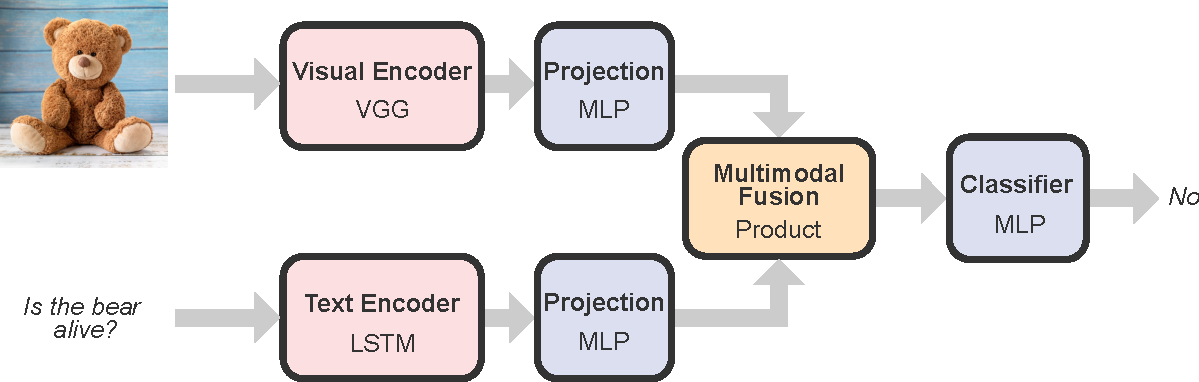
\includegraphics[width=0.8\textwidth]{Figures/Background/vqa_first.pdf}
\caption{First VQA architecture. Image and question embeddings are extracted and then projected to the same dimension. The result is then combined using the element-wise product, and a classifier provides the most likely answer at the output.}
\label{fig:vqa_first}
\end{center}
\end{figure}

Another breakthrough related to attention emerged with \gls{butd} attention~\cite{anderson2018bottom}, where grid features produced by a \gls{cnn} are replaced with object features produced by an \gls{r-cnn}~\cite{ren2015faster}. Attention is then computed along the region features to assign larger weights to the object regions that are more relevant to the question. Later on, \gls{ban} builds on the object-based feature extraction but proposes adding co-attention~\cite{xu2016ask} to \gls{mlb} with the aim of considering the interaction between every object region and every question word.

One of the early signs hinting at the upcoming transition to transformer-based architectures for \gls{vqa} was LXMERT~\cite{tan2019lxmert}. This model comprises three encoder blocks: one for text, one for object relationships, and one to combine both modalities. The cross-modality block has a special design containing a bidirectional cross-attention sub-layer constructed from two uni-directional cross-attention sub-layers, one from text to vision and one from vision to text. LXMERT is notable for being trained on various tasks, including language modeling, masked object prediction, image-text matching, and \gls{vqa}. Between 2020 and 2022, several approaches addressing different aspects of \gls{vqa} were proposed. These include investigating the relevance of grid features against region features~\cite{jiang2020defense}, learning with counterfactuals~\cite{liang2020learning}, data unshuffling~\cite{teney2020unshuffling}, and visual grounding~\cite{khan2021reason}.

Subsequently, the OFA model~\cite{wang2022ofa} emerged as an encoder-decoder transformer with up to 930M parameters, serving, together with Flamingo~\cite{alayrac2022flamingo}, as precursors to \glspl{mllm}, such as GPT-4V~\cite{achiam2023gpt}, BLIP-2~\cite{li2023blip2}, and Llama-adapters~\cite{zhang2023llamaadapter,gao2023llamaadapter}. A significant change introduced by these larger models is their ability to generate free-text answers instead of pre-defined ones, allowing for more varied responses and detailed descriptions.

As depicted in \fig~\ref{fig:vqa_evolution_background}, \glspl{mllm} mark a paradigm shift in the fundamental structure of the \gls{vqa} architecture. As discussed in Sec.~\ref{subsec:mllms}, in numerous state-of-the-art approaches, visual features are extracted with a visual encoder, mapped to the dimension of the language tokens, and then integrated with the language tokens. This facilitates the seamless utilization of the \gls{llm}, which can also be left frozen during the training process~\cite{guo2023images}. More recent advancements in \gls{vqa} focus on adding specialized world knowledge into the model~\cite{wang2024qa} and using synthetic questions to answer human questions~\cite{kim2024generalizing}. 

\subsubsection{Medical VQA}

In the medical domain, the evolution of \gls{medvqa} has closely paralleled the progress made for natural images, with some approaches being directly adapted to the medical domain. \gls{medvqa} is considered to have started later than general \gls{vqa} (see \fig~\ref{fig:vqa_evolution_background}), likely attributed, as mentioned earlier, to limited data availability and the associated annotation costs. The initiation of \gls{medvqa} was significantly influenced by the ImageCLEF VQA-Med challenge, inaugurated in 2018, marking the initial applications of \gls{vqa} to medical images. With a relatively small dataset with only 5,500 question-answer pairs for training, most of the approaches in the challenges were adapted from general \gls{vqa}, such as \gls{san}, \gls{mcb} and \gls{mfb}~\cite{ImageCLEFVQA_Med2018}. Addressing the challenge of limited data, a method was proposed in~\cite{nguyen2019overcoming}, utilizing meta-learning and a \gls{dae} to generalize in limited-data scenarios and exploit unlabeled images, respectively.

Two methods were then introduced for generating answers using different modules based on the type of question asked, either open-ended or close-ended~\cite{zhan2020medical,gupta2021hierarchical}. These practices posed a significant challenge in the early years of \gls{medvqa}, where certain methods were specifically tailored to the challenge data. Some approaches even treated the \gls{vqa} problem as an image classification problem, disregarding the input questions~\cite{al2020inception}. Fortunately, as new datasets emerged, approaches shifted focus towards other aspects, including enhancing the importance assigned to questions~\cite{vu2020question} and incorporating data augmentation techniques~\cite{gong2021cross}. From this point on, the adoption of transformer-based architectures, adapted from general \gls{vqa}, became prominent in \gls{medvqa}. This transition began with a pathology \gls{vqa} model that employed a transformer to fuse text and visual features~\cite{naseem2022vision}. Later, the integration of \glspl{mllm} into \gls{medvqa} has been observed~\cite{vansonsbeek2023openended,seenivasan2023surgicalgpt,he2024pefomed}.

\subsection{Datasets}
\label{sec:vqa_datasets}

In terms of datasets, significant differences exist between general and medical \gls{vqa}. \fig~\ref{fig:vqa_datasets_evolution} shows the most relevant datasets for natural and medical images over time. A notable characteristic of datasets in general \gls{vqa} is the refinement of earlier versions, exemplified by the progression from VQA v1~\cite{antol2015vqa} to VQA v2~\cite{goyal2017making}. Additionally, new versions like VQA-CP~\cite{agrawal2018don} were introduced to mitigate biases. This kind of dataset evolution is hardly observed in the medical domain, where, with some exceptions, there is only one version of the dataset. Due to the lack of data, challenges such as ImageCLEF VQA-Med have also re-used the same dataset used in previous versions~\cite{ImageCLEF-VQA-Med2021}.

\begin{figure}[t]
\begin{center}
\includegraphics[width=\textwidth]{Figures/Background/vqa_datasets_evolution.pdf}
\caption{Evolution of VQA datasets for natural and medical images over time. Dots with triangles and squares indicate datasets produced for a specific VQA challenge.}
\label{fig:vqa_datasets_evolution}
\end{center}
\end{figure}

Perhaps the most important dataset consideration is the number of images and question-answer pairs. As mentioned earlier, data collection in the medical domain is more challenging, resulting in substantially smaller datasets compared to their counterparts in general \gls{vqa}. 

To illustrate this, Table~\ref{tab:datasets_vqa} provides an overview of publicly available \gls{vqa} datasets for medical and natural images. Two conclusions can be drawn: (1) General \gls{vqa} datasets tend to contain more images and more questions than \gls{medvqa} datasets, and (2) \gls{medvqa} datasets often incorporate automatically generated questions. Both of these considerations can be seen as consequences of the difficulties associated with medical data, as presented in Sec.~\ref{subsec:vqa_vs_medvqa}. The first consideration impacts the quality of the models trained with such data, as achieving generalization becomes more challenging, making them more prone to biases. The second consideration limits the applicability or deployment of \gls{medvqa} models in clinical environments, primarily due to the disparity between the nature of automatically generated questions and human-generated questions. Generally, automatically generated questions tend to adhere to a fixed structure that does not fully capture the semantic and syntactic variability and complexity of questions posed by humans. 




\section{Basics of Diabetic Macular Edema (DME) Staging}

We briefly present basic concepts about fundus imaging and \gls{dme} staging due to its relevance in this thesis. \fig~\ref{fig:eye_anatomy} (left) shows the basic anatomy of the eye. This organ exhibits a layered organization crucial for vision. Light initially passes through the transparent cornea, refracting and entering the anterior chamber filled with aqueous humor. The iris, the pigmented structure visible as eye color, regulates the incoming light via the central pupil. The crystalline lens, located behind the iris, further focuses the light onto the retina, the light-sensitive layer lining the posterior chamber. Within the retina, photoreceptor cells, known as rods and cones, convert light energy into electrical signals. These signals are then transmitted through the optic nerve to the visual cortex in the brain, allowing for visual perception. The entire globe of the eye is encased by the tough, white sclera, providing structural support and protection. This intricate interplay of structures enables the eye to capture and process visual information, transforming light into the world we see~\cite{zhu2012eye}.

\begin{table}[ht]
\begin{center}
\begin{tabular}{lp{0.5cm}lp{0.5cm}lp{0.5cm}l}
\toprule
Dataset                       && \# Images         && \# Questions && QA creation \\ \midrule
E-VQA~\cite{yang2023event} && 2,690 && 9,088 && Automatic \\
OK-VQA~\cite{marino2019okvqa}   && 14,031           && 14,055 && Manual \\
VizWiz 2018~\cite{gurari2018vizwiz} && 21,173 && 31,173 && Manual \\
TextVQA~\cite{singh2019towards}   && 28,408           && 45,336 && Manual\\ 
DocVQA~\cite{mathew2021docvqa}   && 12,000           && 50,000 && Manual \\
LoRA~\cite{gao2024lora} && 100,00 && 200,000 && Automatic\\
Visual7W~\cite{zhu2016visual7w}  && 47,300 && 327,929 && Manual \\ 
VQA-CPv1~\cite{agrawal2018don}   && 205,000           && 370,000  && Manual\\
VQAv1~\cite{antol2015vqa}      && 204,721    && 614,163    && Manual  \\ 
VQA-CPv2~\cite{agrawal2018don}   && 219,000          && 658,000  && Manual\\
CLEVR~\cite{johnson2017clevr}   && 100,000 && 864,968   && Automatic \\ 
VQAv2~\cite{goyal2017making}   && 204,721 && 1'105,904 && Manual \\ 
GQA~\cite{hudson2019gqa}  && 113,000           && 22'000,000   &&  Automatic \\ \midrule
RadVisDial (gold)~\cite{kovaleva2020towards}  && 100 && 500 &&  Manual \\ 
VQA-RAD~\cite{lau2018dataset}  && 316 && 3,515 && Manual \\ 
VQA-Med 2020~\cite{ImageCLEF-VQA-Med2020}  && 5,000    &&  5,000 &&  Automatic   \\  
VQA-Med 2021~\cite{ImageCLEF-VQA-Med2021}  && 5,000 && 5,000 && Automatic \\ 
VQA-Med 2018~\cite{ImageCLEFVQA_Med2018} && 2,866    &&   6,413  && Automatic   \\  
DME-VQA~\cite{tascon2022consistency} && 679 && 12,159 && Automatic \\
Slake~\cite{liu2021slake}  && 642 && 14,000 && Manual \\
VQA-Med 2019~\cite{ImageCLEFVQA-Med2019}   && 4,200 &&  15,292 && Automatic \\ 
VQA-Med 2023~\cite{ImageCLEF2023}  && 5,000 && 25,000 && Automatic \\ 
PathVQA~\cite{he2020pathvqa}  && 4,998 && 32,799 && Automatic\\ 
PMC-VQA~\cite{zhang2023pmc}  && 149,000 && 227,000 && Automatic\\ 
RadVisDial (silver)~\cite{kovaleva2020towards}  && 91,060 && 455,300 &&  Automatic \\ \bottomrule
\end{tabular}
\end{center}
\caption{Overview of VQA dataset size sorted by the number of questions. \textbf{Top:} For natural images. \textbf{Bottom:} For medical images.}
\label{tab:datasets_vqa}
\end{table}

\begin{figure}[h]
\begin{center}
\includegraphics[width=\textwidth]{Figures/Background/anatomy_fundus.png}
\caption{\textbf{Left:} Anatomy of the eye (from~\cite{sightresearchukYourEyes}). \textbf{Right:} Fundus image from the IDRiD dataset~\cite{idrid} with hard exudates encircled in light blue.}
\label{fig:eye_anatomy}
\end{center}
\end{figure}

\subsection{Fundus Imaging}

In \gls{dme} risk grade diagnosis from fundus images we are interested in capturing the rear of the eye, which is also known as fundus. This requires a specialized camera focused on the eye while emitting a bright light source, typically a flash or an infrared beam. The light travels through the eye, as described before, and reflects off the structures at the back of the eye and travels back through the pupil. A series of mirrors and lenses within the camera capture and concentrate this reflected light.
Modern fundus cameras are digital, capturing an image directly onto a sensor instead of using film~\cite{bernardes2011digital}. 


\subsection{DME Staging}

In assessing the severity of \gls{dme} through color fundus images, a simplified classification system utilizes a three-point scale (0-2) to categorize disease progression. Grade 0 signifies a healthy retina, devoid of any visible "hard exudates," which appear as yellowish-white deposits. Grade 1 indicates the presence of these deposits confined to the peripheral regions of the retina, outside the central "macular area." Conversely, Grade 2 denotes the presence of hard exudates within the critical macular region, raising potential concerns for vision impairment. For practical purposes, the critical macular region is defined by a circle with a radius of one optic disc diameter~\cite{ren2018diabetic}. \fig~\ref{fig:eye_anatomy} (right) shows an example where hard exudates are within this critical region, leading to Grade 2.
